\documentclass[paper=a4, parskip=half-]{scrartcl}
\usepackage[utf8]{inputenc}

\usepackage{amsmath}
\usepackage{mathtools}
\usepackage{amssymb} % more icons/symbols
\usepackage{hyperref} % for hyper links
\usepackage{graphicx}

\usepackage{geometry}
 \geometry{
 a4paper,
 left=20mm,
 right=20mm,
 top=20mm,
 bottom=30mm,
 }


\title{Applied Cryptography}
\author{\texttt{thgoebel@ethz.ch}}
\date{ETH Zürich, FS 2021}

% Custom commands
\newcommand{\setzeroone}{\lbrace 0, 1 \rbrace} % => {0,1} (Notice the missing $$)
\newcommand{\horizontaldivider}{\begin{center} \line(1,0){350} \end{center}}
\newcommand{\xor}{\oplus}
\newcommand{\A}{\mathcal{A}} % quick access to fancy letters
\newcommand{\C}{\mathcal{C}}
\newcommand{\K}{\mathcal{K}}
\newcommand{\M}{\mathcal{M}}
\newcommand{\adv}{\mathbf{Adv}}


\begin{document}

\begin{titlepage}
\maketitle
\vspace{5cm}
\thispagestyle{empty}


\begin{abstract}
This documents is a \textbf{short} summary for the course \textit{Applied Cryptography} at ETH Zurich.
It is intended as a document for quick lookup, e.g. during revision, and as such does not replace reading the slides or a proper book.

We do not guarantee correctness or completeness, nor is this document endorsed by the lecturers.
Feel free to point out any erratas.
\end{abstract}

\end{titlepage}

\tableofcontents
\newpage
\listoffigures
%\listoftables

Credits: images are generally taken from the lecture slides.
\newpage


\section{Symmetric Cryptography}

\paragraph{One-time pad}
Plaintext $p$, key $k$ such that $|p| = |k|$.
Ciphertext $c = p \xor k$.

If $k$ u.a.r. and only used once then the OTP is \textbf{perfectly secure}, i.e.
$ \Pr[P=p|C=c] = \Pr[P=p]$.

Note: keys can re-occur (as a result of random sampling) but they must not be re-used (i.e. the adversary must not be aware that the same key is used).

Issues: same lengths, key distribution, single use.

\subsection{Block Ciphers}

\paragraph{Block cipher}
A block cipher with key length $k$ and block size $n$ consists of two efficiently computable permutations\footnote{Encipher and decipher}:
$$ E: \setzeroone^k \times \setzeroone^n \mapsto \setzeroone^n \quad
D: \setzeroone^k \times \setzeroone^n \mapsto \setzeroone^n $$
such that for all keys $K$ $D_K$ is the inverse of $E_K$
(where we write $E_K$ short for $E(K, \cdot)$).

\paragraph{Security notions}
Known plaintext attack, chosen plaintext attack, chosen ciphertext attack.
Exhaustive key search on $(P,C)$ pairs -- no attack should be better, else we throw the cipher away.

\paragraph{Pseudo-randomness}
\begin{itemize}
\item Adversary $\A$ interacts either with block cipher $(E_K, D_K)$ or a truly random permutation $(\Pi, \Pi^{-1})$.
\item A block cipher is called a \textbf{pseudo-random permutation PRP} if no efficient\footnote{Quantified by runtime + number of oracle queries.} $\A$ can tell the difference between $E_K$ and $\Pi$ (no access to the inverse).
\item A block cipher is called a \textbf{strong-PRP} if no efficient $\A$ can tell the difference between $(E_K, D_K)$ and $(\Pi, \Pi^{-1})$.
\end{itemize}

\begin{figure}[h]
    \centering
	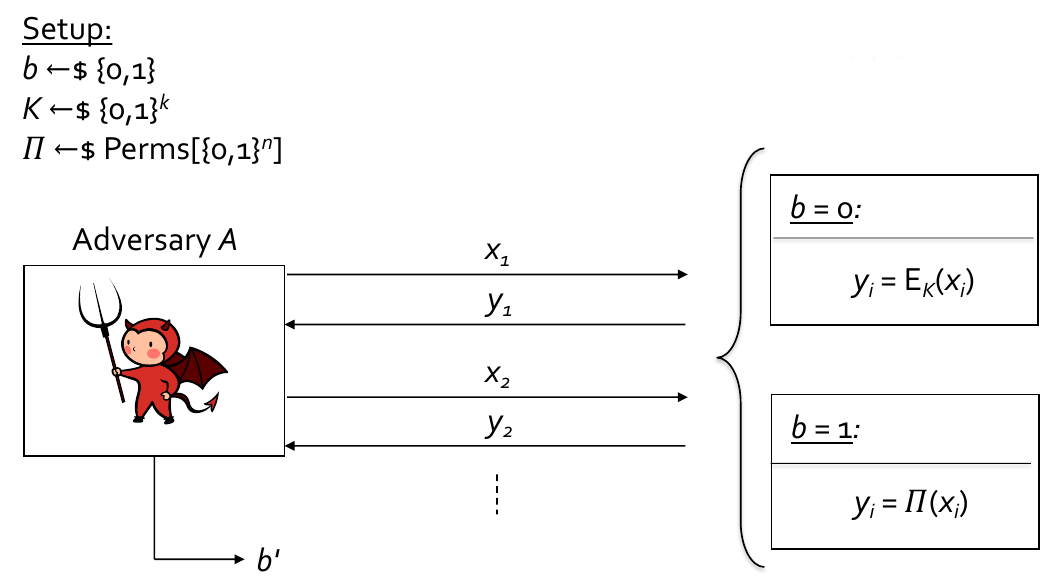
\includegraphics[scale=0.4]{images/prp.png}
    \caption{PRP game}
    \label{fig:prp}
\end{figure}

The advantage is defined as:
$$
\mathbf{Adv}^{PRP}_E (\A)
= 2 \cdot \Big| \Pr[ \text{Game }\textbf{PRP}(\A, E) \Rightarrow \text{true} ] - \frac{1}{2} \Big|
$$
where the probability is over the randomness of $b, K, \Pi, \A$.
Note that $\Pr[ \text{Game }\textbf{PRP}(\A, E) \Rightarrow \text{true} ] = \Pr[b'=b]$.

\paragraph{Constructing block ciphers}
In general: keyed round function that is repeated many times.

\begin{itemize}
\item Feistel cipher: halved blocks crossing back and forth, e.g. DES
\item Substitution-permutation network: confusion + diffusion, e.g. AES
\end{itemize}

\paragraph{Electronic Code Book (ECB) mode}
Same plaintext always maps to the same ciphertext (deterministic).
Thus serious leakage, don't use.

\begin{figure}[h]
    \centering
	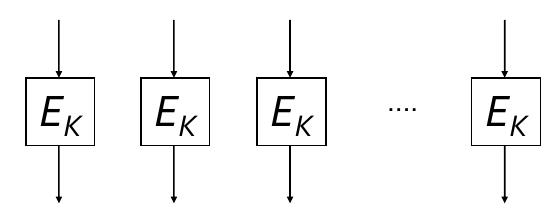
\includegraphics[scale=0.4]{images/ecb.png}
    \caption{ECB mode}
    \label{fig:ecb}
\end{figure}

\paragraph{Cipher Block Chaining (CBC) mode}
Use u.a.r. IV/previous ciphertext block to randomise encryption.

A bit flip in $C_i$ completely scrambles/randomises $P_i$ and flips the same bit in $P_{i+1}$.

Caveats: non-random IV, padding oracle attack, ciphertext block collisions (after using the same key for $2^{n/2}$ blocks by the birthday bound).

\begin{figure}[h]
    \centering
	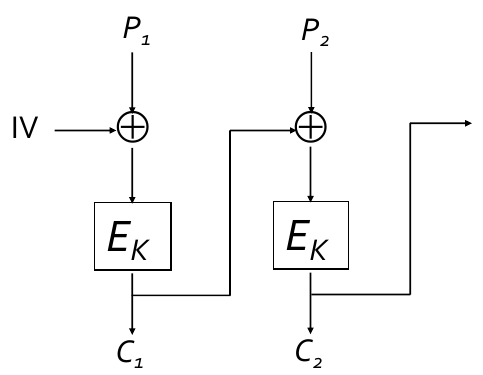
\includegraphics[scale=0.4]{images/cbc-enc.png}
	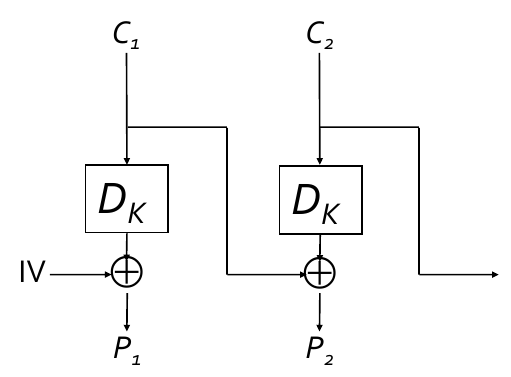
\includegraphics[scale=0.4]{images/cbc-dec.png}
    \caption{CBC mode (left: encipher, right: decipher)}
    \label{fig:cbc}
\end{figure}

\paragraph{Counter (CTR) mode}
Incrementing counter is encrypted with block cipher to produce a pseudo-random value to xor the plaintext block with.

Effectively a stream cipher producing OTP keys.
$E_K$ does not even need to be invertible.
No padding needed, can just truncate the last block.
A bit flip it $C_i$ flips the same bit in $P_i$.

Caveats: counter must not repeat/wrap around (else xor of ciphertexts = xor of plaintexts).

\begin{figure}[h]
    \centering
	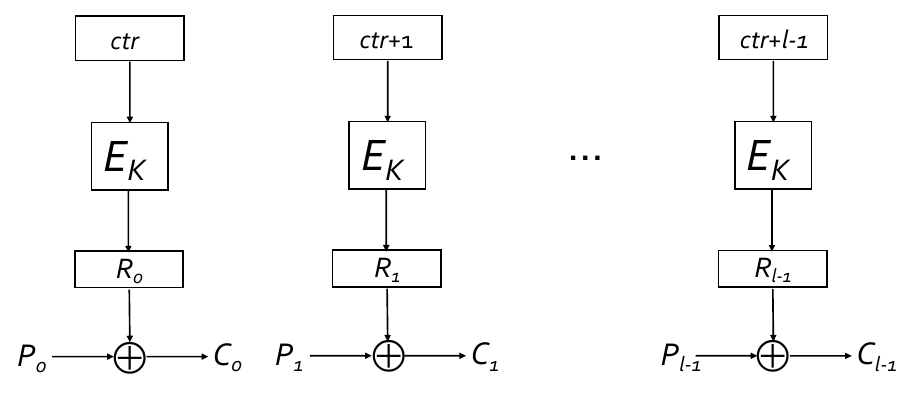
\includegraphics[scale=0.4]{images/ctr.png}
    \caption{CTR mode}
    \label{fig:ctr}
\end{figure}


\subsection{Symmetric Encryption}

\paragraph{Symmetric Encryption Scheme}
is a triple $ SE = (KGen, Enc, Dec) $.
We have key space $\K = \setzeroone^k$, message space $\M = \setzeroone^*$\footnote{In reality we might have a maximum plaintext length.} and ciphertext space $\C = \setzeroone^*$.
For correctness, we have $ Dec_K(Enc_K(m))=m $.

\paragraph{IND-CPA Security}
Informally:
computational version of perfect security --
an efficient adversary cannot compute anything useful from a ciphertext (e.g. hide every bit of the plaintext.
Equivalent to \emph{semantic security}.

Formally:
For any efficient adversary $\A$, given the encryption of one of two equal-length messages of its choice,
$\A$ is unable to distinguish which one of the two messages was encrypted.

In the security game, $\A$ gets access to a \emph{Left-or-Right encryption oracle}.
The advantage of $\A$ is:
$$
\adv^{IND-CPA}_{SE} (\A)
= 2 \cdot \Big| \Pr[ \text{Game }\textbf{IND-CPA}(\A, SE) \Rightarrow \text{true} ] - \frac{1}{2} \Big|
$$

Notes:
Deterministic schemes \textbf{cannot} be IND-CPA secure (why?).
CBC and CTR mode (if used properly) can be proven to be IND-CPA secure (assuming that $Enc$ is a PRP-secure block cipher).

Caveats:
No integrity. Says nothing about messages of non-equal length. No chosen ciphertexts.

\begin{figure}[h]
    \centering
	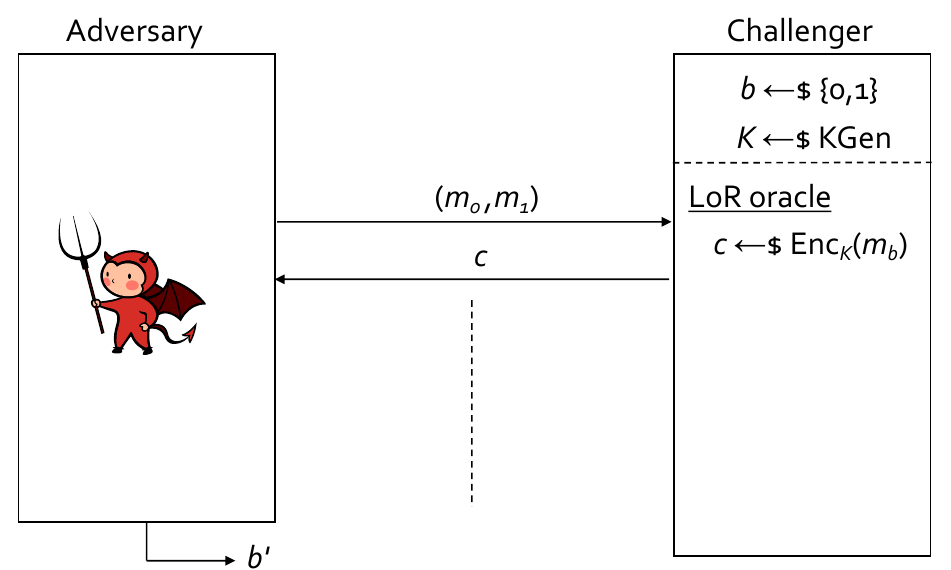
\includegraphics[scale=0.4]{images/ind-cpa.png}
    \caption{IND-CPA game}
    \label{fig:ind-cpa}
\end{figure}

\paragraph{Advantage Rewriting Lemma}
Let $b$ be a uniformly random bit and $b'$ the output of some algorithm. Then:
$$
2 \Big| \Pr[b'=b] - \frac{1}{2} \Big| = \Big| \Pr[b'=1|b=1] - \Pr[b'=1|b=0] \Big|
$$

\paragraph{Difference Lemma}
Let $Z, W_1, W_2$ be events. If
$$
(W_1 \wedge \neg Z) \text{ occurs if and only if } (W_2 \wedge \neg Z) \text{ occurs}
$$
then
$$
\Big| \Pr[W_2] - \Pr[W_1] \Big| \leq \Pr[Z]
$$
In practice: $Z$ is a bad event that rarely happens, $W_1, W_2$ are when $\A$ wins in security games $G_1, G_2$.
Useful for \emph{game hopping} proofs.

\paragraph{PRP-PRF Switching Lemma}
Let $E$ be a block cipher.
Then for any algorithm $\A$ making $q$ queries:
$$
\Big| \adv^{PRP}_{E} (\A) - \adv^{PRF}_{E} (\A) \Big| \leq \frac{q^2}{2^{n+1}}
$$



\subsection{Hash Functions}


\subsection{Message Authentication Codes MACs}


\subsection{Authenticated Encryption}


\newpage


\section{Asymmetric Cryptography}

\subsection{TODO}

\paragraph{TODO} 
 

\newpage


\section{Advanced Cryptography}

\subsection{Data at rest}

\subsubsection{Searchable Encryption}

\paragraph{Searchable Encryption}
consists of three protocols:
\begin{enumerate}
\item Setup:
Client generates an \emph{encrypted database + encrypted search index}%
\footnote{A search index is a mapping from document ids to keywords, and/or vice versa.
For more details see the lecture \textit{Information Retrieval}.},
uploads them to the server.
\item Search:
Client generates a \emph{search token}, server uses it to process the search, returns the result.
\item Update:
Client generates an \emph{update token}, server uses it to update the encrypted database and encrypted search index, returns success/failure.
\end{enumerate}
%
Active field of research, many open problems (e.g. leakage analysis + prevention).

\paragraph{Goals}
\begin{itemize}
\item Security:
Confidentiality (of data and queries) against an \emph{honest-but-curious} server.%
\footnote{Compare this security model against a fully malicious server.}
\item Efficiency:
Storage, computational, bandwidth requirements.
\item Functionality:
Supported query types.
\end{itemize}

\paragraph{First construction}
Idea: randomly choose a PRF $F_K$ and replace each keyword $w$ in the index by $F_K(w)$.
Also encrypt each document under some symmetric key $K_0$.

Leakage from setup $\mathcal{L}_{Setup}$:
total number of documents and keywords, keyword frequency, co-occurences of keywords.

Leakage from searches $\mathcal{L}_{Search}$:
result patterns, query patterns, result intersection between queries.

\begin{figure}[h]
    \centering
	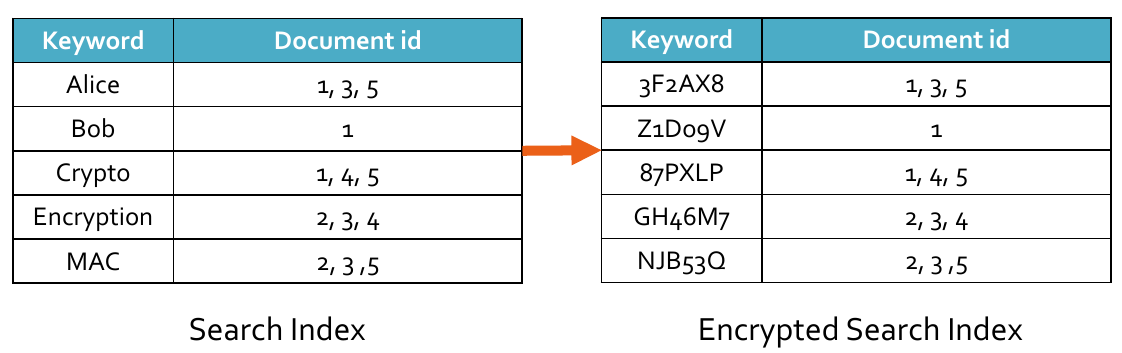
\includegraphics[scale=0.4]{images/searchable-encryption-1.png}
    \caption{First construction for searchable encryption}
    \label{fig:searchable-encryption-1}
\end{figure}

\paragraph{Second construction}
Idea: randomly choose a PRF $F_K$.
For each keyword $w$ calculate $K_1 || K_2 = F_K(w)$.
Replace each keyword with $K_1$ (as before).
In addition: associate each document id for $w$ with a counter $cnt$ and replace the id with $id \xor F_{K_2}(cnt)$.

This hides the co-occurences of keyword pairs (PRF security).

\begin{figure}[h]
    \centering
	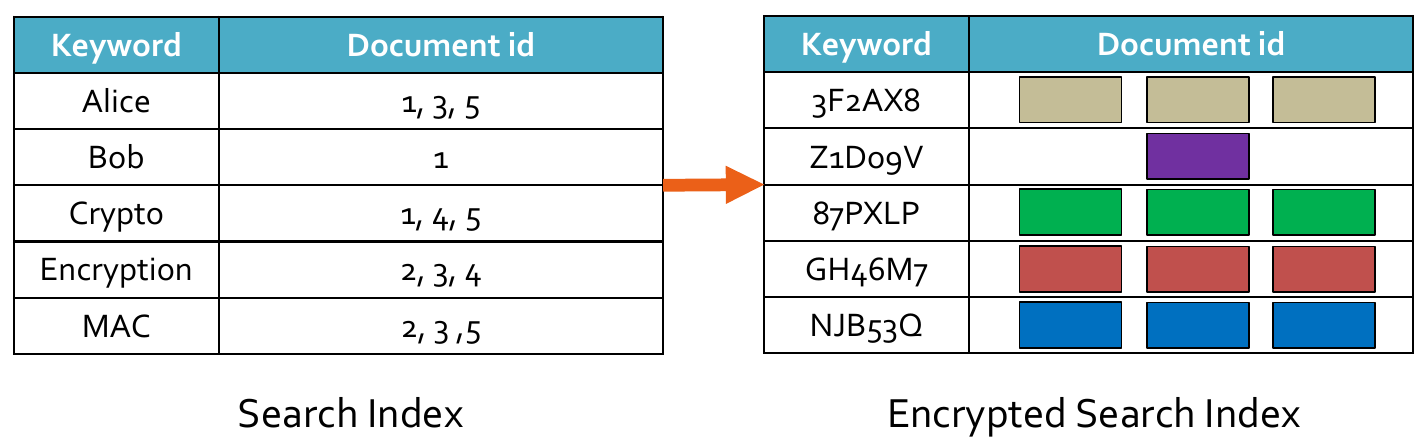
\includegraphics[scale=0.35]{images/searchable-encryption-2.png}
    \caption{Second construction for searchable encryption}
    \label{fig:searchable-encryption-2}
\end{figure}

\paragraph{Third construction}
Idea: ... (as before) ... \\
In addition: associate each document id for $w$ with a counter $cnt$ and replace the id with $id \xor F_{K_2}(cnt)$.
Then store this document id value in a key-value store (dictionary) under ``key'' $F_{K_1}(cnt)$.

Search:
Send $(K_1, K_2, |cnt_{querystring}|)$ to the server.
Server recomputes the $F_{K_1}(cnt)$ to find the values in the dictionary.
Then decrypts them to document ids using $K_2$.
Looks up the encrypted documents and returns them.

Leakage from setup $\mathcal{L}_{Setup}$:%
\footnote{This is also what an adversary learns from a single snapshot.}
total number of documents.

Leakage from searches $\mathcal{L}_{Search}$:
(same as before) result patterns, query patterns, result intersection between queries.

\begin{figure}[h]
    \centering
	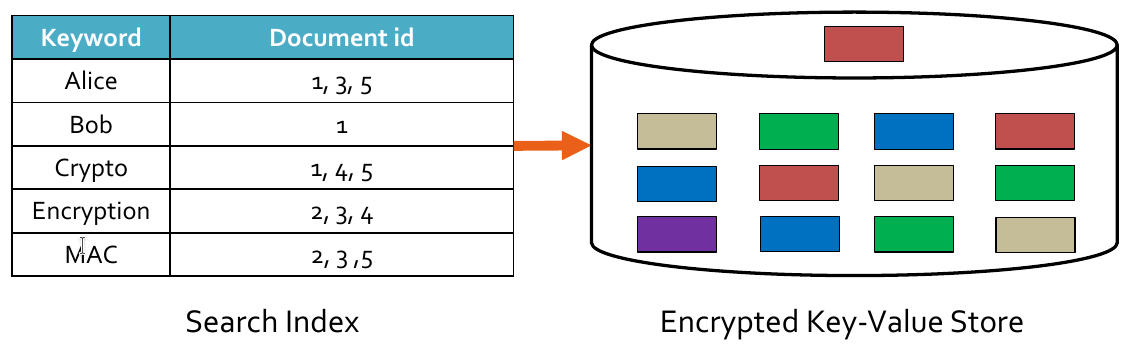
\includegraphics[scale=0.4]{images/searchable-encryption-3.png}
    \caption{Third construction for searchable encryption (setup)}
    \label{fig:searchable-encryption-3}
\end{figure}
\begin{figure}[h]
    \centering
	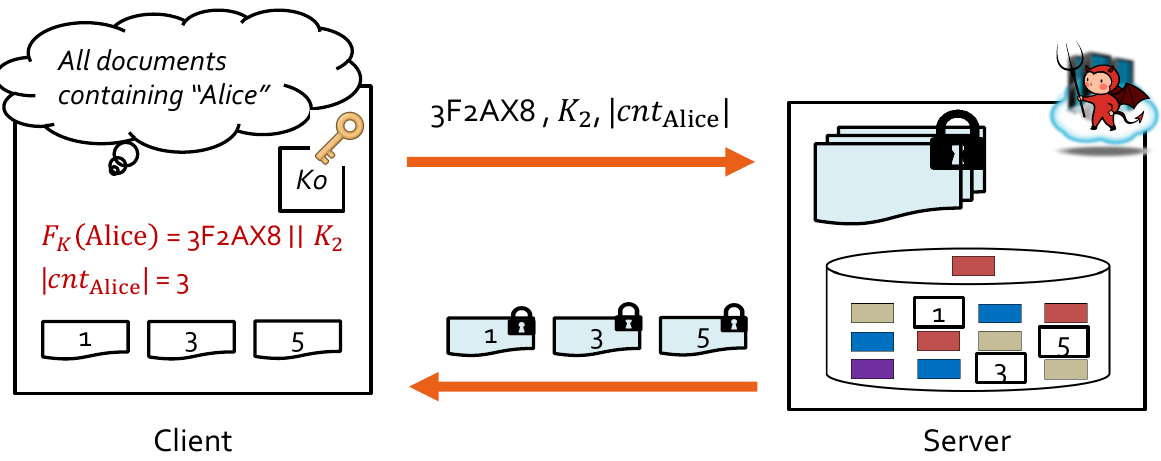
\includegraphics[scale=0.4]{images/searchable-encryption-4.png}
    \caption{Third construction for searchable encryption (search)}
    \label{fig:searchable-encryption-4}
\end{figure}

\paragraph{Defining Leakage}
Goal: formally define the leakage $\mathcal{L} = (\mathcal{L}_{Setup}, \mathcal{L}_{Search})$ of searchable encryption schemes.

Security game: an adversary $\A$ interacts with a challenger $\C$ that contains either the real world or a simulator.
The simulator $\mathcal{S}$ only has access to the leakage $\mathcal{L}$ (but not to the secret key).
Intuitively, the adversary should gain no extra information other than the leakage.

\begin{figure}[h]
    \centering
	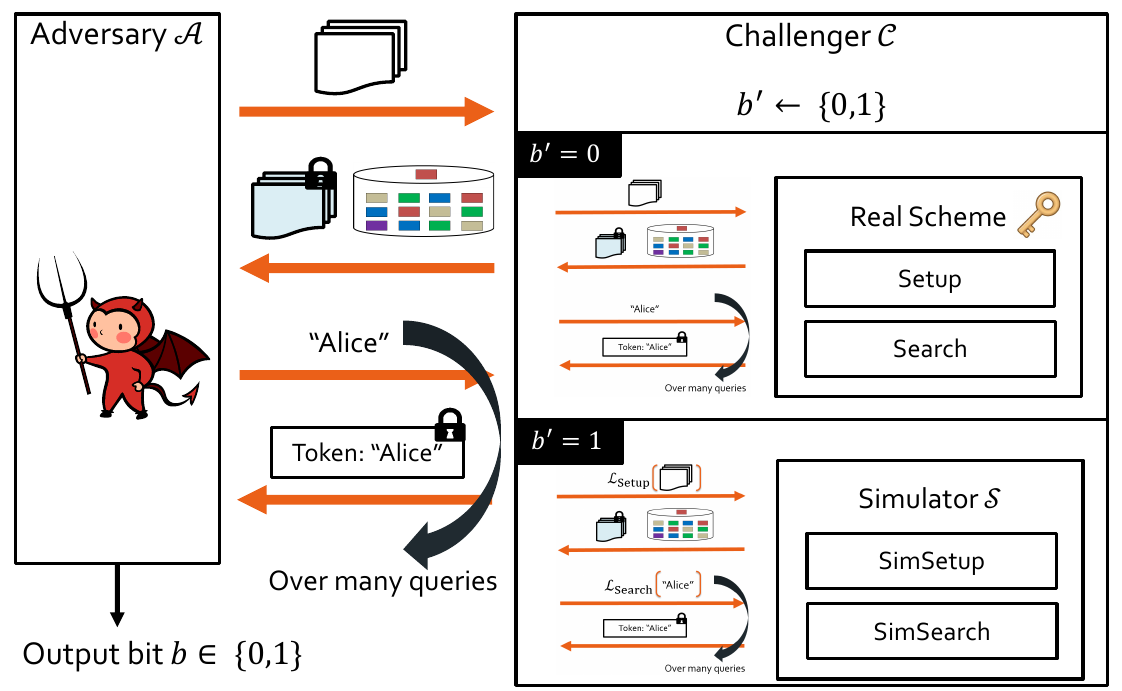
\includegraphics[scale=0.4]{images/searchable-encryption-leakage.png}
    \caption{Searchable encryption leakage game}
    \label{fig:searchable-encryption-leakage}
\end{figure}

\paragraph{Analysing Leakage}
What can the adversary infer from the leakage?
It turns out that given auxiliary information, one can e.g. perform query recovery.


\subsection{Data in transit}

\subsubsection{Transport Layer Security TLS}

TODO


\subsubsection{Signal Messaging Protocol}

TODO


\subsubsection{Messaging Layer Security Protocol}

TODO


\subsection{Data under computation}

\subsubsection{Fully Homomorphic Encryption FHE}

\paragraph{Motivation}
Allow data to be processed while remaining encrypted.
Applications: Secure Outsourcing, Private Set Intersection (PSI), Private Machine Learning As A Service.

\paragraph{Challenges}
\begin{itemize}
\item Crypto: Underlying math, parameter selection, security analysis.
\item Computation Paradigm: No if/else, no loops, no jumps -- all would leak
information about the encrypted data. Optimisations, approximations, SIMD batching.
\end{itemize}

\paragraph{(Ring-) Learning With Errors (R)LWE}
The LWE problem is conjectured to be hard (even on quantum computers).
Simplified idea: mask data with random noise.
Need to carefully define encryption/decryption, addition and multiplication.
For multiplication, we need \emph{relinearization} to make the maths work.

Problem: noise increases with each operation and will eventually grow too large for decryption to succeed.
Solution: use \emph{bootstrapping} to (homomorphically) reduce the noise again.
Effectively, bootstrapping produces an encryption of the same encrypted message,
but at a lower noise level.\footnote{This is one of the practical breakthroughs of Gentry '09.}
But: bootstrapping is complex and slow (order of seconds to minutes), so we try to avoid it in practice.

\begin{figure}[h]
    \centering
	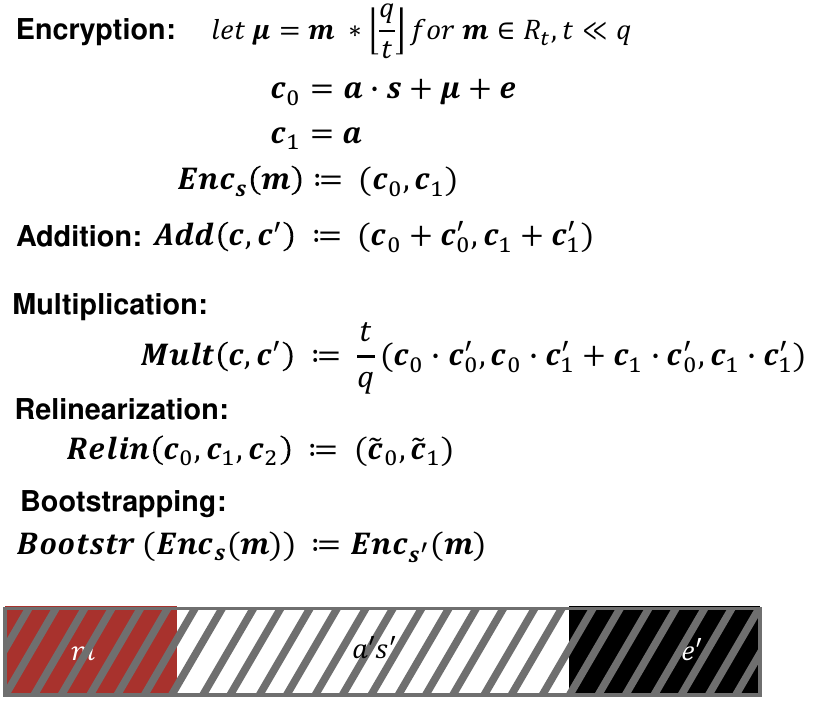
\includegraphics[scale=0.4]{images/fhe-rlwe.png}
    \caption{FHE: RLWE operations}
    \label{fig:fhe-rlwe}
\end{figure}

\paragraph{Parameter selection}
Careful trade-off between efficiency, security and correctness.
Security based on current knowledge on how hard the LWE problem is.

\paragraph{Tool support}
``Libraries'' implement the underlying FHE schemes, addressing the crypto side.
``Compilers'' help with writing higher-level code, addressing the computation paradigm concerns.
E.g. SEAL (C++), EVA (Python), nGraph-HE (Tensorflow), SEALion (Keras).


\newpage

\end{document}
